% textidote: ignore begin
\section{Chess}\label{sec:chess}
% textidote: ignore end

Chess is a game that has existed for millennia.
It has roots in India as well as China where the first iterations of chess we know today was invented~\cite{murray1913}.

Nowadays, the chess standard universally known as chess is the iteration of the game called international chess or
western chess, which is also the standard that FIDE, the international chess governing body, uses~\cite{fide2024}.

Most people are familiar with chess, hereby the rules of the game and the look of the board.
We will therefore only mention a few key elements of chess and online chess, which are not as common knowledge and will
be important for the final product.

\subsection{Notation}\label{subsec:notation}

Notation in chess regards how one is able to communicate the events of a particular game in writing.
The modern standard is the algebraic notation, where the rows are named from `1' through `8' going from white to black
and the columns are named from `a' through `h' going from queen-side to king-side.
As an example, the notation `a1' refers to the bottom left cell from white's perspective~\cite{pickel2022}.

As seen in Figure~\ref{fig:chess-notation-example}, when moving, one specifies the piece to be moved and the
destination.
In the line labeled `1' only the destination is mentioned in both moves, which implies that it was pawn moves.
In the line labeled `4' there is an `x' implying the capture of another piece as a result of the move.

% textidote: ignore begin
\begin{figure}[h]
    \centering
    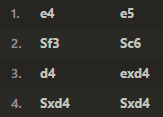
\includegraphics[width=0.5\textwidth]{chess-notation-example}
    \caption{Chess notation example~\cite{chess.com2024}}.\label{fig:chess-notation-example}
\end{figure}
% textidote: ignore end

This notation style is efficient and is also the way computers write and read moves.
The \lstinline{pgn} file extension is used for text files that encapsulates completed chess games.
Only one game is stored per file~\cite{chess.com2024}.

% textidote: ignore begin

\subsection{Rules}\label{subsec:rules}
% textidote: ignore end

Another important aspect of the game of chess is the more complicated rules.
Below we will mention a few of the important more scarcely known rules:

\begin{itemize}
    \item \textbf{Time control}: Different tournaments and types of games have different time control rules, such as
    rewarding time after every move.
    Another example is the game type Armageddon, where black and white have different starting times on the clock~\cite{schiller2012}.
    \item \textbf{Draw}: Drawing or tying in chess can happen in different ways.
    Examples include stalemate, the 50 move rule and repetition~\cite{schiller2012}.
    \item \textbf{En passant}: A pawn can capture another pawn, if the second mentioned pawn was moved by a double move
    to either adjacent side of the first mentioned pawn~\cite{schiller2012}.
\end{itemize}
